\documentclass[journal]{IEEEtran}
\usepackage{listings}
\usepackage{amssymb}
\usepackage{algpseudocode}
\usepackage{color}

% *** GRAPHICS RELATED PACKAGES ***
%
\ifCLASSINFOpdf
  \usepackage[pdftex]{graphicx}
  
  
\else

\fi

\begin{document}

\title{K-Means Clustering}

\author{Preston Engstrom}

% make the title area
\maketitle
\lstset{language=Python}

% As a general rule, do not put math, special symbols or citations
% in the abstract or keywords.
\begin{abstract}
The K-Means clustering algorithm has been a mainstay of unsupervised machine learning for decades. The algorithm is explored in this report using known datasets of 2D points, using several cluster counts and distance measures, with results compared using the Dunn Index for cluster analysis.
\end{abstract}


\begin{IEEEkeywords}
Clustering, K-means, Machine Learning
\end{IEEEkeywords}

\IEEEpeerreviewmaketitle


\section{Introduction}
\IEEEPARstart{T}{he} K-Means Clustering Algortihm has continued to be the workhorse of clustering tasks since its development in 1967 by James MacQueen.
In this implementation, the data consists of points on a 2D plain. The clusters are simply the collection of points closest to the center of the cluster based on some distance measure. K-means, and clustering algorithms in general, suffer greatly from the curse of dimensionallity due to their reliance on relating data vectors to each other in a multidimensional space. Presenting data in a 2D space is the best case scenario for exploring the behavior of the algorithm. 

\subsection{Problem Definition}
 Clustering is the task of grouping a set of unlabled data vectors into groups, or clusters. Items in a cluster should be more alike items in the same cluster, and much less like items in other clusters. Clustering is one of the most common tasks of exploratory data mining for extracting preliminary observations about datasets. This paper begins with a description of the K-Means Algorithm and its implementation using the Euclidean, Chebyshev and Minkowski distance measures. The results are then presented and compared using the Dunn Index.



\section{The K-Means Algorithm}
K-Means is a method of vector quantization taken from signal processing. Vector quantization itself is the process of taking a set of complex vectors and compressing them into broader group. With its origins for lossy data compression and lossy error correction, the same processes have been applied for data exploration, pattern recognition and clustering, as in K-Means.

The K-Means alogrithm can be divided into 2 distinct steps. The assignment step and the update step, where the centroids are moved and member data points updated until convergence is reached.



\subsection{Description}
K-Means begins with an initial set of K centroids, wich serve as the centers of each cluster. The assignment step can be expressed as follows[7]:

$$ S_{i}^{(t)} = \{x_{p}: ||x_{p} -m_{i}^{(t)}||^{2 } \leq  ||x_{p} -m_{j}^{(t)}||^{2 } \ \forall j, 1 \leq j \leq k\} $$


Where each data vector $ x_{p} $ is assigned to exactly one cluster $S_{i}$ based on, in the case of this representation, the smallest euclidean distance to the closest mean $m_{i} ....m_{j}$. For each group, the mean of the member data vectors is then calculated, and the clusters centroid is then moved to that position:
$$m_{i}^{t+1} = \frac{1}{|S_{i}^{(t)}|}\Sigma x_{j}$$
This is run for each centroid $x_{j}$. These steps, assignment and update, are repeated until no change occurs between two assignment steps. This convergence generally happens quite quickly, but can scale exponentially with the number of dimensions.


\subsection{Centroid Intialization }

\subsection{Pseudocode Implementation}
\begin{figure}
	\caption{Simple Backprop Skeleton}
	\begin{lstlisting}
	given training example and label
	for each training example:
	
	for o in outputs:
	calculate output_delta
	
	for h in hidden:
	calculate hidden delta
	
	update hidden weights
	update input weights
	\end{lstlisting}
\end{figure}

\subsection{Distance Measures}

\subsection{Euclidean Distance}

\subsection{Chebyshev Distance}

\subsection{Minkowski Distance}
\section{Cluster Analysis Using The Dunn Index}



\section{Results and Discussion}
\begin{table}[h]
	\renewcommand{\arraystretch}{1.3}
	
	\caption{Comparison of S-Set Dunn Index, Euclidian Distance}
	\label{table_example}
	\centering
	
	\begin{tabular}{|c|c|c|c|c|}
		\hline
		Dataset & 10 Centroids & 15 Centroids & 20 Centroids & Optimal Value\\
		\hline
		
		S1 & 0.004797  & 0.012200 & 0.005278 & 0.0367893\\
		\hline
		S2 & 0.002901 & 0.005611 & 0.006178 & 0.020947\\
		\hline
		S3 & 0.006027 & 0.008156 & 0.008058 & 0.004394\\
		\hline
		S4 & 0.005708 & 0.006873 & 0.005099 & 0.007474\\
		\hline
	\end{tabular}
\end{table}

\begin{figure}[!t]
\centering
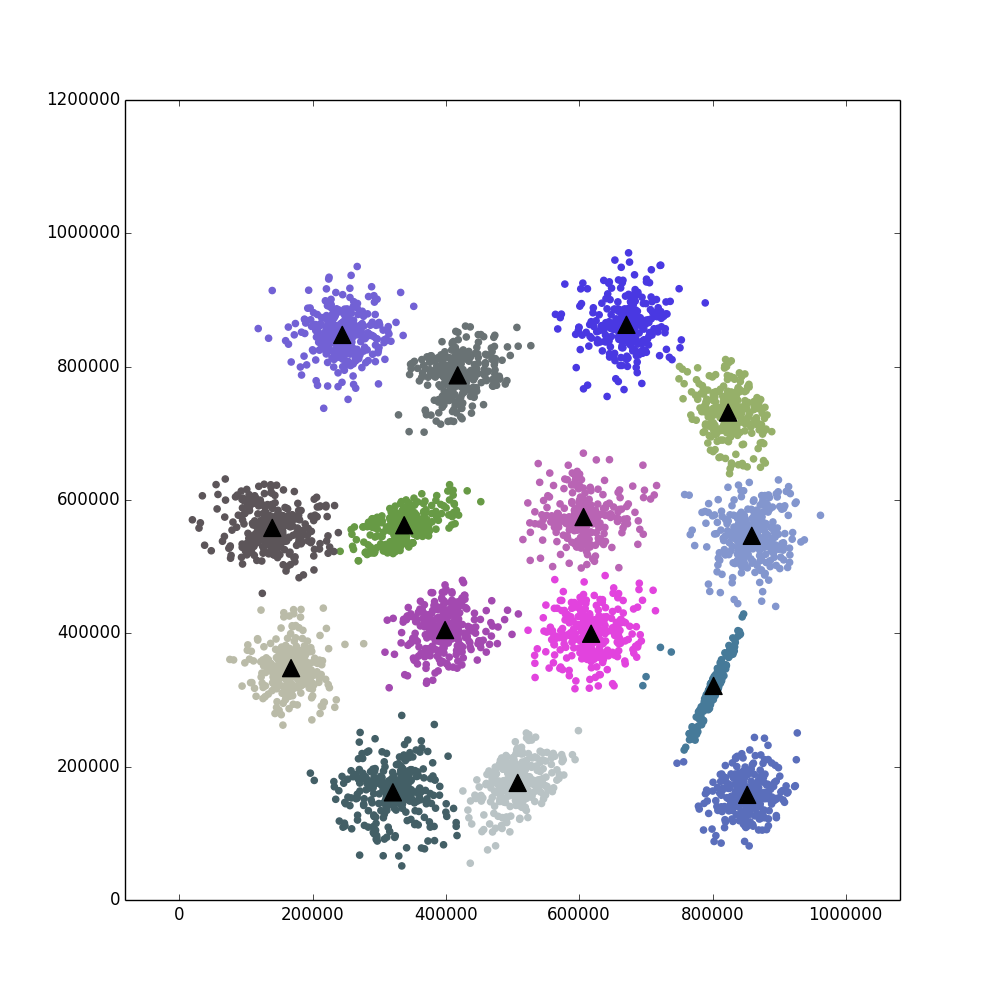
\includegraphics[width=2.5in]{../figs/s1_true_euclid_15.png}
\caption{Optimal Clusters for the S1 dataset.}
\label{fig_sim}
\end{figure}

\begin{figure}[!t]
	\centering
	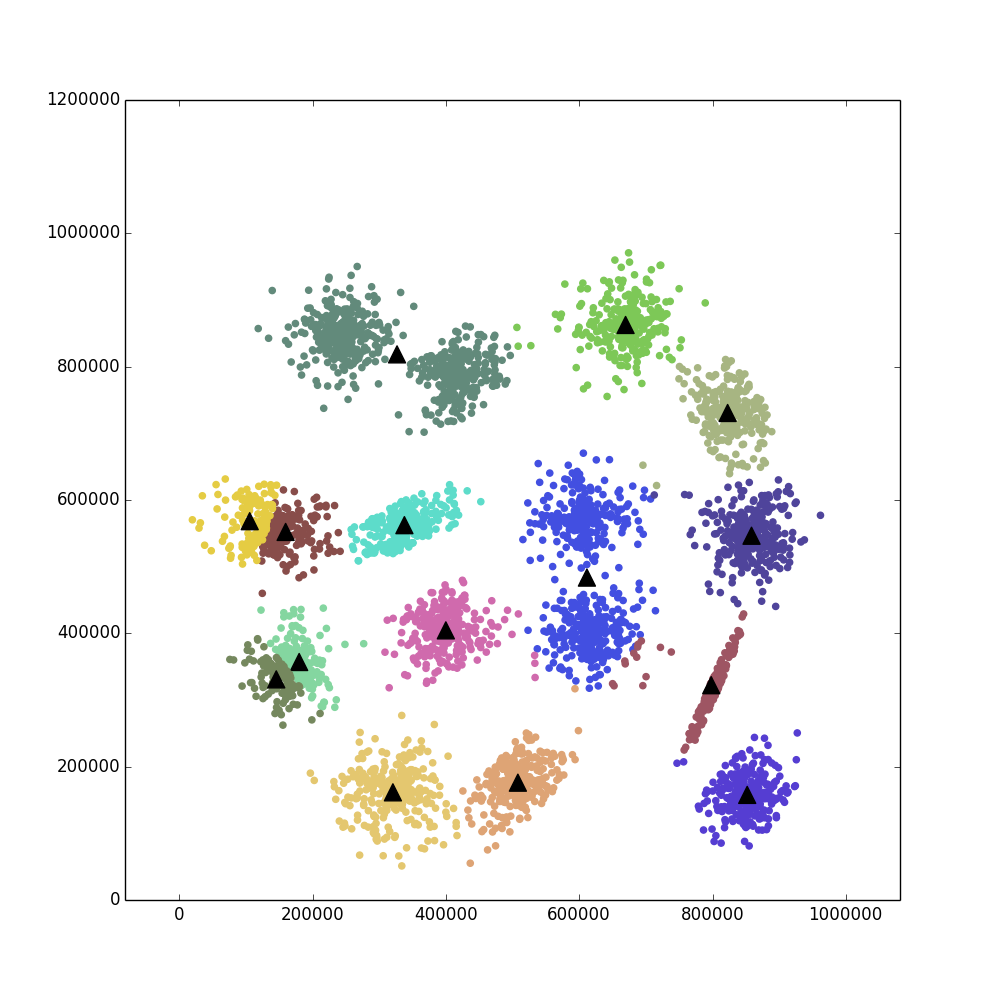
\includegraphics[width=2.5in]{../figs/s1_rand_euclid_15.png}
	\caption{Results using 15 randomly initialized centroids on the S1 Dataset.}
	\label{fig_sim}
\end{figure}

\begin{figure}[!t]
	\centering
	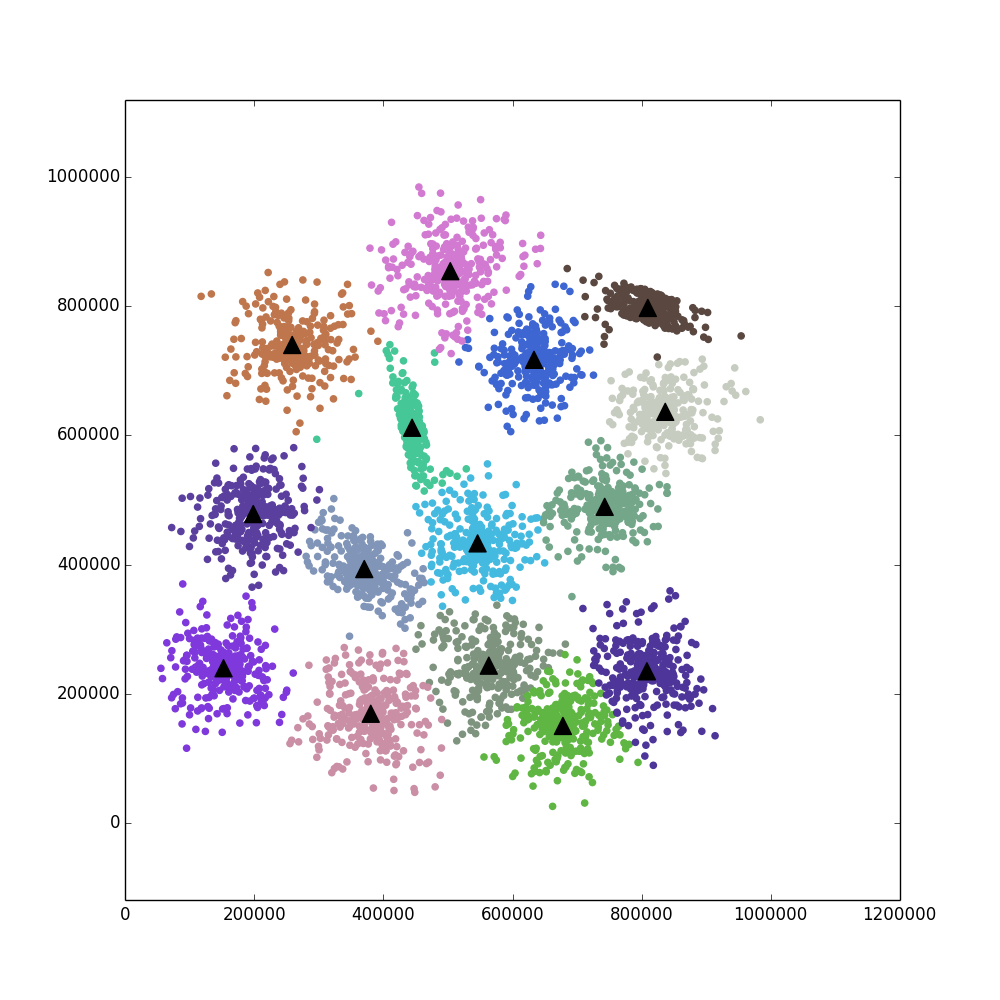
\includegraphics[width=2.5in]{../figs/s2_true_euclid_15.png}
	\caption{Optimal Clusters for the S2 dataset.}
	\label{fig_sim}
\end{figure}


\begin{figure}[!t]
	\centering
	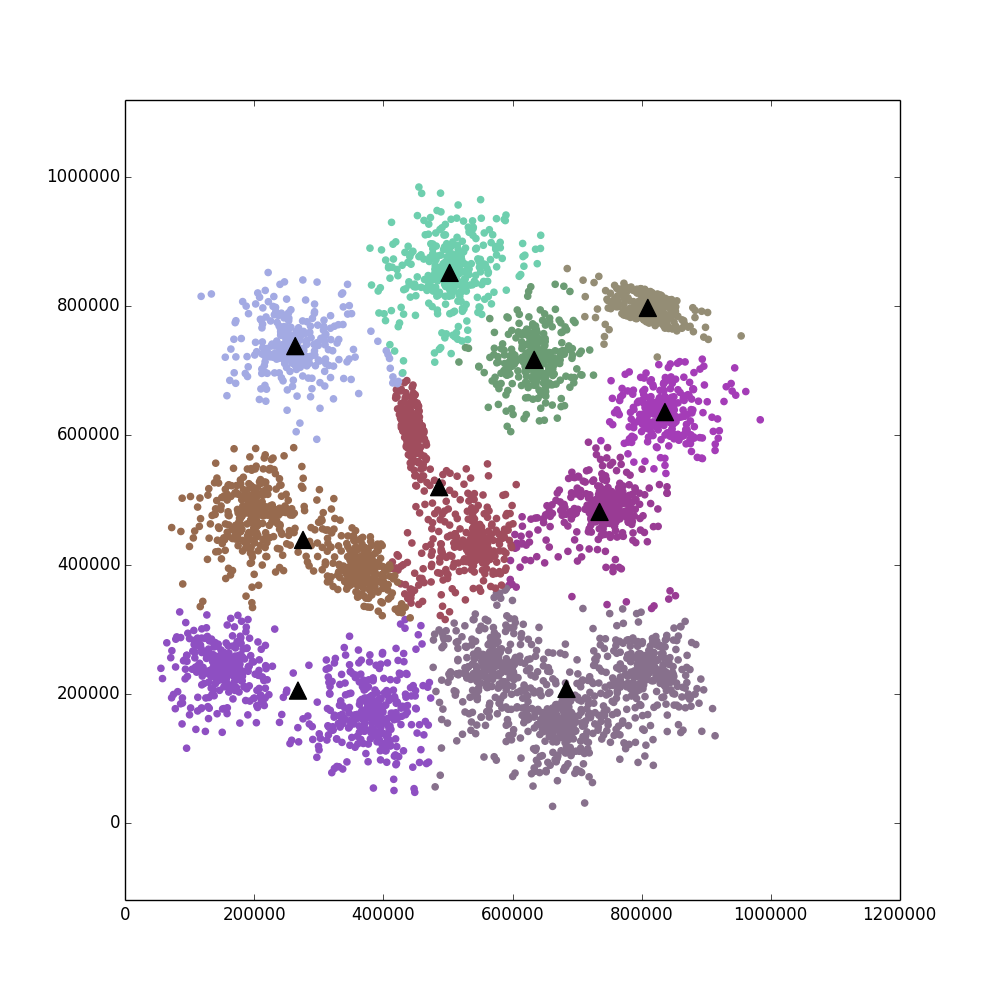
\includegraphics[width=2.5in]{../figs/s2_rand_euclid_10.png}
	\caption{Results using 10 randomly initialized centroids on the S2 Dataset.}
	\label{fig_sim}
\end{figure}




\section{Conclusion}


The conclusion goes here.

\ifCLASSOPTIONcaptionsoff
  \newpage
\fi
\begin{thebibliography}{1}
	
	\bibitem{IEEEhowto:kopka}
 [1]D. MacKay, Information theory, inference, and learning algorithms. Cambridge, UK: Cambridge University Press, 2003.
\end{thebibliography}



% that's all folks
\end{document}


